
\documentclass[letterpaper,hide notes,xcolor={table,svgnames},pdftex,10pt]{beamer}
\def\showexamples{t}


%\usepackage[svgnames]{xcolor}

%% Demo talk
%\documentclass[letterpaper,notes=show]{beamer}

\usecolortheme{crane}
\setbeamertemplate{navigation symbols}{}

\usetheme{MyPittsburgh}
%\usetheme{Frankfurt}

%\usepackage{tipa}

\usepackage{hyperref}
\usepackage{graphicx,xspace}
\usepackage[normalem]{ulem}

\newcommand\SF[1]{$\bigstar$\footnote{SF: #1}}

\usepackage[default]{sourcesanspro}
\usepackage[T1]{fontenc}

\newcounter{tmpnumSlide}
\newcounter{tmpnumNote}

% old question code
%\newcommand\question[1]{{$\bigstar$ \small \onlySlide{2}{#1}}}
% \newcommand\nquestion[1]{\ifdefined \presentationonly \textcircled{?} \fi \note{\par{\Large \textbf{?}} #1}}
% \newcommand\nanswer[1]{\note{\par{\Large \textbf{A}} #1}}


 \newcommand\mnote[1]{%
   \addtocounter{tmpnumSlide}{1}
   \ifdefined\showcues {~\tiny\fbox{\arabic{tmpnumSlide}}}\fi
   \note{\setlength{\parskip}{1ex}\addtocounter{tmpnumNote}{1}\textbf{\Large \arabic{tmpnumNote}:} {#1\par}}}

\newcommand\mmnote[1]{\note{\setlength{\parskip}{1ex}#1\par}}

%\newcommand\mnote[2][]{\ifdefined\handoutwithnotes {~\tiny\fbox{#1}}\fi
% \note{\setlength{\parskip}{1ex}\textbf{\Large #1:} #2\par}}

%\newcommand\mnote[2][]{{\tiny\fbox{#1}} \note{\setlength{\parskip}{1ex}\textbf{\Large #1:} #2\par}}

\newcommand\mquestion[2]{{~\color{red}\fbox{?}}\note{\setlength{\parskip}{1ex}\par{\Large \textbf{?}} #1} \note{\setlength{\parskip}{1ex}\par{\Large \textbf{A}} #2\par}\ifdefined \presentationonly \pause \fi}

\newcommand\blackboard[1]{%
\ifdefined   \showblackboard
  {#1}
  \else {\begin{center} \fbox{\colorbox{blue!30}{%
         \begin{minipage}{.95\linewidth}%
           \hspace{\stretch{1}} Some space intentionally left blank; done at the blackboard.%
         \end{minipage}}}\end{center}}%
         \fi%
}



%\newcommand\q{\tikz \node[thick,color=black,shape=circle]{?};}
%\newcommand\q{\ifdefined \presentationonly \textcircled{?} \fi}

\usepackage{listings}
\lstset{%
  keywordstyle=\bfseries,
  aboveskip=15pt,
  belowskip=15pt,
  captionpos=b,
  identifierstyle=\ttfamily,
  escapeinside={(*@}{@*)},
  stringstyle=\ttfamiliy,
  frame=lines,
  numbers=left, basicstyle=\scriptsize, numberstyle=\tiny, stepnumber=0, numbersep=2pt}

\usepackage{siunitx}
\newcommand\sius[1]{\num[group-separator = {,}]{#1}\si{\micro\second}}
\newcommand\sims[1]{\num[group-separator = {,}]{#1}\si{\milli\second}}
\newcommand\sins[1]{\num[group-separator = {,}]{#1}\si{\nano\second}}
\sisetup{group-separator = {,}, group-digits = true}

%% -------------------- tikz --------------------
\usepackage{tikz}
\usetikzlibrary{positioning}
\usetikzlibrary{arrows,backgrounds,automata,decorations.shapes,decorations.pathmorphing,decorations.markings,decorations.text}

\tikzstyle{place}=[circle,draw=blue!50,fill=blue!20,thick, inner sep=0pt,minimum size=6mm]
\tikzstyle{transition}=[rectangle,draw=black!50,fill=black!20,thick, inner sep=0pt,minimum size=4mm]

\tikzstyle{block}=[rectangle,draw=black, thick, inner sep=5pt]
\tikzstyle{bullet}=[circle,draw=black, fill=black, thin, inner sep=2pt]

\tikzstyle{pre}=[<-,shorten <=1pt,>=stealth',semithick]
\tikzstyle{post}=[->,shorten >=1pt,>=stealth',semithick]
\tikzstyle{bi}=[<->,shorten >=1pt,shorten <=1pt, >=stealth',semithick]

\tikzstyle{mut}=[-,>=stealth',semithick]

\tikzstyle{treereset}=[dashed,->, shorten >=1pt,>=stealth',thin]

\usepackage{ifmtarg}
\usepackage{xifthen}
\makeatletter
% new counter to now which frame it is within the sequence
\newcounter{multiframecounter}
% initialize buffer for previously used frame title
\gdef\lastframetitle{\textit{undefined}}
% new environment for a multi-frame
\newenvironment{multiframe}[1][]{%
\ifthenelse{\isempty{#1}}{%
% if no frame title was set via optional parameter,
% only increase sequence counter by 1
\addtocounter{multiframecounter}{1}%
}{%
% new frame title has been provided, thus
% reset sequence counter to 1 and buffer frame title for later use
\setcounter{multiframecounter}{1}%
\gdef\lastframetitle{#1}%
}%
% start conventional frame environment and
% automatically set frame title followed by sequence counter
\begin{frame}%
\frametitle{\lastframetitle~{\normalfont(\arabic{multiframecounter})}}%
}{%
\end{frame}%
}
\makeatother

\makeatletter
\newdimen\tu@tmpa%
\newdimen\ydiffl%
\newdimen\xdiffl%
\newcommand\ydiff[2]{%
    \coordinate (tmpnamea) at (#1);%
    \coordinate (tmpnameb) at (#2);%
    \pgfextracty{\tu@tmpa}{\pgfpointanchor{tmpnamea}{center}}%
    \pgfextracty{\ydiffl}{\pgfpointanchor{tmpnameb}{center}}%
    \advance\ydiffl by -\tu@tmpa%
}
\newcommand\xdiff[2]{%
    \coordinate (tmpnamea) at (#1);%
    \coordinate (tmpnameb) at (#2);%
    \pgfextractx{\tu@tmpa}{\pgfpointanchor{tmpnamea}{center}}%
    \pgfextractx{\xdiffl}{\pgfpointanchor{tmpnameb}{center}}%
    \advance\xdiffl by -\tu@tmpa%
}
\makeatother
\newcommand{\copyrightbox}[3][r]{%
\begin{tikzpicture}%
\node[inner sep=0pt,minimum size=2em](ciimage){#2};
\usefont{OT1}{phv}{n}{n}\fontsize{4}{4}\selectfont
\ydiff{ciimage.south}{ciimage.north}
\xdiff{ciimage.west}{ciimage.east}
\ifthenelse{\equal{#1}{r}}{%
\node[inner sep=0pt,right=1ex of ciimage.south east,anchor=north west,rotate=90]%
{\raggedleft\color{black!50}\parbox{\the\ydiffl}{\raggedright{}#3}};%
}{%
\ifthenelse{\equal{#1}{l}}{%
\node[inner sep=0pt,right=1ex of ciimage.south west,anchor=south west,rotate=90]%
{\raggedleft\color{black!50}\parbox{\the\ydiffl}{\raggedright{}#3}};%
}{%
\node[inner sep=0pt,below=1ex of ciimage.south west,anchor=north west]%
{\raggedleft\color{black!50}\parbox{\the\xdiffl}{\raggedright{}#3}};%
}
}
\end{tikzpicture}
}


%% --------------------

%\usepackage[excludeor]{everyhook}
%\PushPreHook{par}{\setbox0=\lastbox\llap{MUH}}\box0}

%\vspace*{\stretch{1}

%\setbox0=\lastbox \llap{\textbullet\enskip}\box0}

\setlength{\parskip}{\fill}

\newcommand\noskips{\setlength{\parskip}{1ex}}
\newcommand\doskips{\setlength{\parskip}{\fill}}

\newcommand\xx{\par\vspace*{\stretch{1}}\par}
\newcommand\xxs{\par\vspace*{2ex}\par}
\newcommand\tuple[1]{\langle #1 \rangle}
\newcommand\code[1]{{\sf \footnotesize #1}}
\newcommand\ex[1]{\uline{Example:} \ifdefined \presentationonly \pause \fi
  \ifdefined\showexamples#1\xspace\else{\uline{\hspace*{2cm}}}\fi}

\newcommand\ceil[1]{\lceil #1 \rceil}


\AtBeginSection[]
{
   \begin{frame}
       \frametitle{Outline}
       \tableofcontents[currentsection]
   \end{frame}
}



\pgfdeclarelayer{edgelayer}
\pgfdeclarelayer{nodelayer}
\pgfsetlayers{edgelayer,nodelayer,main}

\tikzstyle{none}=[inner sep=0pt]
\tikzstyle{rn}=[circle,fill=Red,draw=Black,line width=0.8 pt]
\tikzstyle{gn}=[circle,fill=Lime,draw=Black,line width=0.8 pt]
\tikzstyle{yn}=[circle,fill=Yellow,draw=Black,line width=0.8 pt]
\tikzstyle{empty}=[circle,fill=White,draw=Black]
\tikzstyle{bw} = [rectangle, draw, fill=blue!20, 
    text width=4em, text centered, rounded corners, minimum height=2em]
    
    \newcommand{\CcNote}[1]{% longname
	This work is licensed under the \textit{Creative Commons #1 3.0 License}.%
}
\newcommand{\CcImageBy}[1]{%
	\includegraphics[scale=#1]{creative_commons/cc_by_30.pdf}%
}
\newcommand{\CcImageSa}[1]{%
	\includegraphics[scale=#1]{creative_commons/cc_sa_30.pdf}%
}
\newcommand{\CcImageNc}[1]{%
	\includegraphics[scale=#1]{creative_commons/cc_nc_30.pdf}%
}
\newcommand{\CcGroupBySa}[2]{% zoom, gap
	\CcImageBy{#1}\hspace*{#2}\CcImageNc{#1}\hspace*{#2}\CcImageSa{#1}%
}
\newcommand{\CcLongnameByNcSa}{Attribution-NonCommercial-ShareAlike}

\newenvironment{changemargin}[1]{% 
  \begin{list}{}{% 
    \setlength{\topsep}{0pt}% 
    \setlength{\leftmargin}{#1}% 
    \setlength{\rightmargin}{1em}
    \setlength{\listparindent}{\parindent}% 
    \setlength{\itemindent}{\parindent}% 
    \setlength{\parsep}{\parskip}% 
  }% 
  \item[]}{\end{list}} 




\title{Lecture 2 --- Review of Computer Architecture}

\author{Jeff Zarnett \\ \small \texttt{jzarnett@uwaterloo.ca}}
\institute{Department of Electrical and Computer Engineering \\
  University of Waterloo}
\date{\today}


\begin{document}

\begin{frame}
  \titlepage

 \end{frame}

\begin{frame}
\frametitle{Computer Organization}

A regular program like a word processor need not be concerned with the underlying hardware of the computer.

The OS must be aware of the details and manage them.

What is a program? Instructions and data.


\end{frame}

\begin{frame}
\frametitle{To Execute a Program}

To execute a program we need:

\begin{enumerate}
	\item \textbf{Main Memory}
	\item \textbf{System Bus}
	\item \textbf{Processor}
\end{enumerate}

Of course, this is the minimal set.

\end{frame}

\begin{frame}
\frametitle{Modern Personal Computer}

\begin{center}
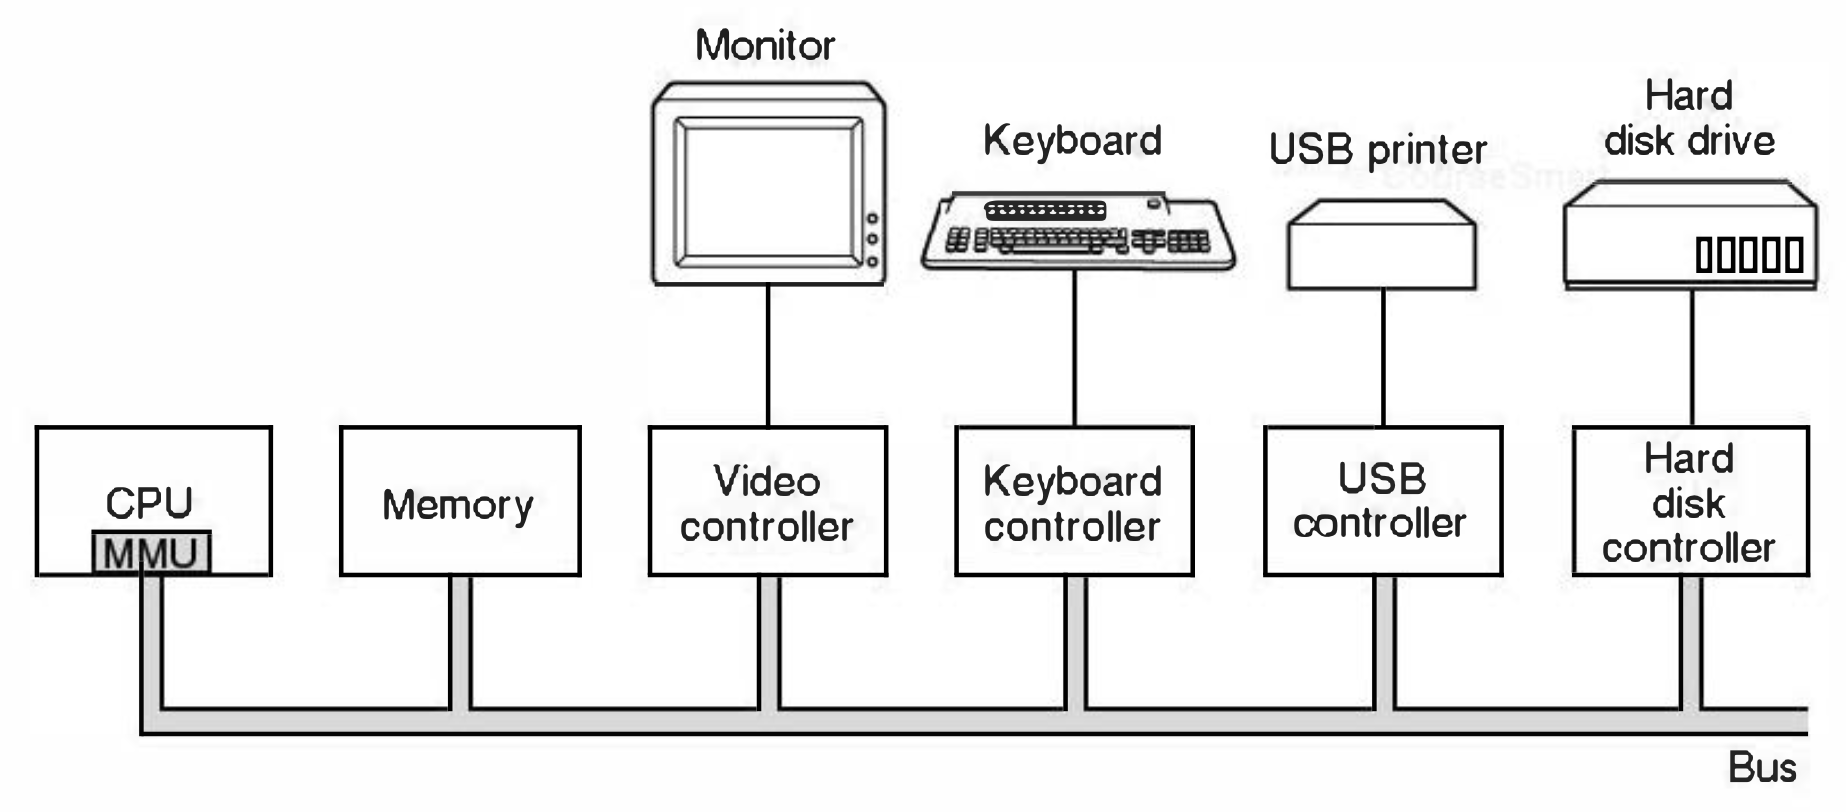
\includegraphics[width=0.8\textwidth]{images/modernpc.png}
\end{center}

A fourth element: \textbf{Input/Output} (I/O). Not strictly necessary, but a computer without it is not very useful...
\end{frame}

\begin{frame}
\frametitle{Main Memory}
Ideally, memory would be:

\begin{itemize}
	\item Fast enough that the processor never has to wait;
	\item Large enough to hold all the data;
	\item Inexpensive.
\end{itemize}

The \alert{Iron Triangle}: ``fast, good, cheap; pick two.''

Good news: we can have different levels of memory.

\end{frame}

\begin{frame}
\frametitle{Main Memory}

Different levels of memory at different sizes, speed, and cost.\\
\quad So what we end up with is a hierarchy of memory.

Let us compare the various levels I might have in my laptop from 2013:

\begin{center}
	\begin{tabular}{l|l|l}
	\textbf{Memory Level} & \textbf{Access Time} & \textbf{Total Capacity} \\ \hline
	Register & 1 ns & < 1 KB \\
	Cache & 2 ns & 6 MB \\
	Main Memory (RAM) & 10 ns & 16 GB \\
	Magnetic Hard Disk & 10 ms & 500 GB \\
	\end{tabular}
\end{center}

Fast memory is expensive!

The difference in access time is often quite dramatic.

\end{frame}

\begin{frame}
\frametitle{Memory Access Analogy}
I am the CPU and a particular book is the piece of data needed.

If the data is in the cache: the book is on a bookshelf in my office.

If the data for the CPU on a magnetic hard disk, I have to get the book from Library and Archives Canada in Ottawa (550 km away).\\
\quad And I would have to walk.

The CPU doesn't go get the data; instead it must wait for it to arrive.

What might I do in the meantime...?

\end{frame}


\begin{frame}
\frametitle{System Buses}

\begin{quote}
	\textit{The bits on the bus go up and down, up and down, up and down...}
\end{quote}


\end{frame}

\begin{frame}
\frametitle{System Buses}

Every sort of communication using the same bus.\\
\quad Contention for this resource is a limiting factor. 

The original IBM PC did work like that.\\
\quad A modern system has numerous buses.

\end{frame}

\begin{frame}
\frametitle{Central Processing Unit (CPU)}

The processor (CPU) is the brain of the computer.

Fetch instructions, decode them, execute them.

Fetch-decode-execute cycle repeated until the program finishes.

Different steps may be completed in parallel (\alert{pipeline}).

Processors' largest unit is the \alert{word}.\\
\quad 32-bit computer $\rightarrow$ 32-bit word. 64-bit computer $\rightarrow$ 64-bit word.

\end{frame}

\begin{frame}
\frametitle{Central Processing Unit (CPU)}
CPU instructions are specific to the processor.

Written assembly? You know the books.

Some operations only available in supervisor mode.\\
\quad Attempting to run it in user mode is an error.


\end{frame}

\begin{frame}
\frametitle{Central Processing Unit (CPU)}
CPUs have storage locations: \alert{registers}.

They may store data or instructions.

Management of registers is partly the role of the OS.

Let us examine a few of the critical registers.

\end{frame}

\begin{frame}
\frametitle{CPU Registers}

A few of the registers in a typical CPU:

\begin{itemize}
	\item \textbf{Program Counter} -- Next instruction.
	\item \textbf{Status Register} -- Array of bits to indicate flags.
	\item \textbf{Instruction Register} -- Instruction most recently fetched.
	\item \textbf{Stack Pointer} -- Top of the stack.
	\item \textbf{General Purpose Registers} -- Store data, addresses, etc.
\end{itemize}


\end{frame}


\begin{frame}
\frametitle{Program Execution}

Program is a sequence of instructions. We can categorize them as:

\begin{enumerate}
	\item \textbf{Processor-Memory}
	\item \textbf{Processor-I/O}
	\item \textbf{Data Processing}
	\item \textbf{Control} 
\end{enumerate}

\end{frame}

\begin{frame}
\frametitle{Interrupts}

If I ordered a book from Ottawa, it takes a long time to arrive.

In the meantime, I should do something else.

Polling: check periodically if the book has arrived.

Interrupts: get a notification when the book is here.

If someone knocks on my door, I pause what I'm doing and get the book.


\end{frame}

\begin{frame}
\frametitle{Sources of Interrupts}

We can put interrupts into four categories, based on their origin:

\begin{enumerate}
	\item \textbf{Program.}
	\item \textbf{Timer.}
	\item \textbf{Input/Output.}
	\item \textbf{Hardware Failure.}
\end{enumerate}


\end{frame}

\begin{frame}
\frametitle{Interrupts}
Interrupts are a way to improve processor utilization.

CPU time is valuable!

When an interrupt take place, the CPU might ignore it (rarely).

More commonly: we need to \alert{handle} it in some way.

Analogy: professor in a lecture; student has a question.


\end{frame}

\begin{frame}
\frametitle{Interrupts}
The OS: stores the state, handles the interrupt, and restores the state.

Sometimes the CPU is in the middle of something uninterruptible.\\
\quad Interrupts may be disabled (temporarily).

Interrupts can have different priorities.
\end{frame}

\begin{frame}
\frametitle{Interrupts}

We may also have multiple interrupts in a short period of time:

\begin{center}
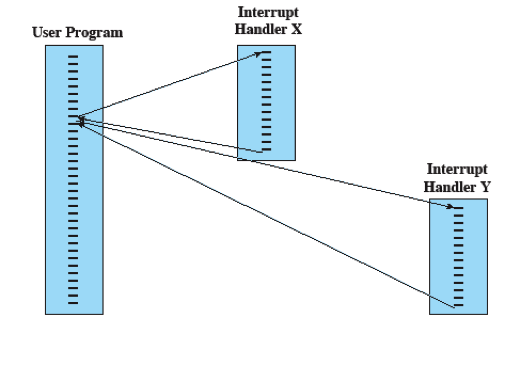
\includegraphics[width=0.45\textwidth]{images/interrupts-sequential.png}
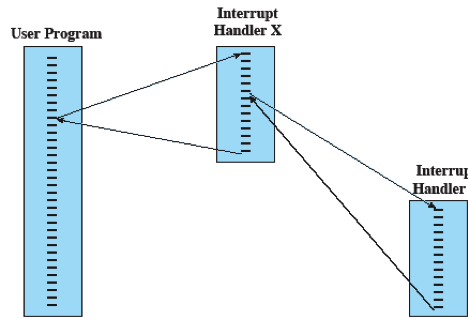
\includegraphics[width=0.45\textwidth]{images/interrupts-nested.png}
\end{center}

They may be sequential (left) or nested (right).

A combination may be used.


\end{frame}

\begin{frame}
\frametitle{Storing and Restoring State}

The OS must store the program state when an interrupt occurs.

The state must be stored.

State: values of registers.

Push them onto the stack.

Interrupt finished: restore the state (pop off the stack).

Then execution continues.

\end{frame}

\begin{frame}
\frametitle{Multiprogramming}
That is saving and restoring the same program.

Why not restore a different program?

We will come to this in scheduling.


\end{frame}


\begin{frame}
\frametitle{I/O Communication}

Three major strategies for communication: 

\begin{enumerate}
	\item \textbf{Programmed I/O.} -- Polling.
	\item \textbf{Interrupt Driven I/O.} -- Interrupts.
	\item \textbf{Direct Memory Access (DMA).} -- CPU does setup.
\end{enumerate}

\end{frame}

\begin{frame}
\frametitle{Direct Memory Access}

The CPU will do some set up, indicating:

\begin{enumerate}
	\item The operation to perform (read or write)
	\item The source
	\item The destination
	\item How much data is to be transferred
\end{enumerate}

This data is sent to the DMA module (a delegate). 

After that, the CPU can go on to do other work.

The I/O device will interact directly with memory.


\end{frame}





\end{document}

